%This section presents \NAME, a \emph{THRee-valued Integrated Verification framEwork}. 
An overview of \NAME\ is presented in Figure~\ref{Fig.3vdv}.
\NAME\ takes as inputs a partial model $M$ and  a property $\phi$ and produces one of the outputs shown by the grey filled shapes.
The outputs are generated by integrating a model checker for partial models and a theorem prover.





The \emph{model checker for partial models} verifies whether the property $\phi$ of interest is definitely satisfied ($\LTLtrue$), possibly satisfied ($?$) or not satisfied ($\LTLfalse$) by the current partial model. 
If the property is \emph{not satisfied} (\circled{3}), there exist some behaviors which definitively violate the property of interest and do not depend on the unspecified parts of the model.
The model checker returns one such behavior, i.e., a definitive counterexample. 
Whenever a property is \emph{definitely satisfied}, its satisfaction does not depend on the unspecified parts, i.e., on how the incomplete parts are later refined.
Finally, if the property is \emph{possibly satisfied} (\circled{5}), the model checker returns a possible counterexample, i.e., a possible violating behavior that the model can exhibit.



The \emph{theorem proving} framework is executed when a $\LTLtrue$ or $?$ value is returned by the model checker and computes a proof which specifies why the property $\phi$ is definitely (possibly) satisfied by $M$.
When a property is \emph{definitely satisfied} (\circled{6}), \NAME\ returns a proof that specifies why the search of a definitive and a possible counterexample has failed. 
Instead, whenever a property is \emph{possibly satisfied} (\circled{4}), besides providing a possible counterexample, \NAME\ returns a proof that specifies why a definitive counterexample has not been found.



\begin{figure}[t]
\begin{center}         
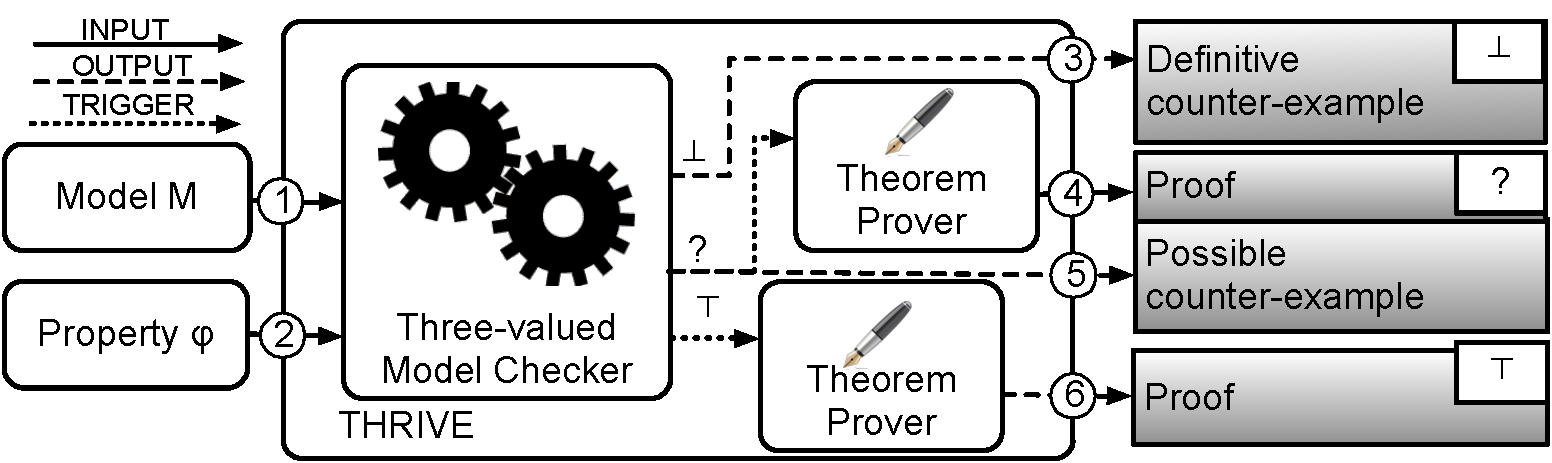
\includegraphics[width=\linewidth]{./images/atvaFig.pdf}
\end{center}
\caption{The \NAME\ framework.}  
\label{Fig.3vdv}
\end{figure}








